% !TeX program = pdfLaTeX
\documentclass[smallextended]{svjour3}       % onecolumn (second format)
%\documentclass[twocolumn]{svjour3}          % twocolumn
%
\smartqed  % flush right qed marks, e.g. at end of proof
%
\usepackage{amsmath}
\usepackage{graphicx}
\usepackage[utf8]{inputenc}

\usepackage[hyphens]{url} % not crucial - just used below for the URL
\usepackage{hyperref}
\providecommand{\tightlist}{%
  \setlength{\itemsep}{0pt}\setlength{\parskip}{0pt}}

%
% \usepackage{mathptmx}      % use Times fonts if available on your TeX system
%
% insert here the call for the packages your document requires
%\usepackage{latexsym}
% etc.
%
% please place your own definitions here and don't use \def but
% \newcommand{}{}
%
% Insert the name of "your journal" with
% \journalname{myjournal}
%

%% load any required packages here
\usepackage{caption}
\usepackage{tabularx}
\usepackage{multirow}
\usepackage{placeins}


% Pandoc citation processing


\begin{document}

\title{Open source landscape ecology tools \thanks{Grants or other notes about the article that should go on the front
page should be placed here. General acknowledgments should be placed at the
end of the article.} }



\author{  Maximillian H.K. Hesselbarth \and  Jakub Nowosad \and  \ldots{} \and  }


\institute{
        Maximillian H.K. Hesselbarth \at
     Department of Ecosystem Modelling, University of Goettingen, Buesgenweg 4, 37077 Goettingen, Germany \\
     \email{\href{mailto:mhk.hesselbarth@gmail.com}{\nolinkurl{mhk.hesselbarth@gmail.com}}}  %  \\
%             \emph{Present address:} of F. Author  %  if needed
    \and
        Jakub Nowosad \at
     Institute of Geoecology and Geoinformation, Adam Mickiewicz University, Krygowskiego 10, 61-680 Poznan, Poland \\
     \email{\href{mailto:nowosad.jakub@gmail.com}{\nolinkurl{nowosad.jakub@gmail.com}}}  %  \\
%             \emph{Present address:} of F. Author  %  if needed
    \and
        \ldots{} \at
     \ldots{} \\
     \email{\ldots{}}  %  \\
%             \emph{Present address:} of F. Author  %  if needed
    \and
    }

\date{Received: date / Accepted: date}
% The correct dates will be entered by the editor


\maketitle

\begin{abstract}
max. (200 words) Abstract Abstract Abstract Abstract Abstract Abstract Abstract Abstract Abstract Abstract Abstract Abstract Abstract Abstract Abstract Abstract Abstract Abstract Abstract Abstract Abstract Abstract Abstract Abstract Abstract Abstract Abstract Abstract Abstract Abstract Abstract Abstract Abstract Abstract Abstract Abstract Abstract Abstract Abstract Abstract Abstract Abstract Abstract Abstract Abstract Abstract Abstract Abstract Abstract Abstract Abstract Abstract Abstract Abstract Abstract Abstract Abstract Abstract Abstract Abstract Abstract Abstract Abstract Abstract Abstract Abstract Abstract Abstract Abstract Abstract Abstract Abstract Abstract Abstract Abstract Abstract Abstract Abstract Abstract Abstract Abstract Abstract Abstract Abstract Abstract Abstract Abstract Abstract Abstract Abstract Abstract Abstract Abstract Abstract Abstract Abstract Abstract Abstract Abstract Abstract
\\
\keywords{
        keyword 1 \and
        keyword 2 \and
        keyword 3 \and
        keyword 4 \and
        \ldots{} \and
    }


\end{abstract}


\def\spacingset#1{\renewcommand{\baselinestretch}%
{#1}\small\normalsize} \spacingset{1}


\hypertarget{sec:intro}{%
\section{Introduction}\label{sec:intro}}

\hypertarget{sec:landscape_ecology}{%
\subsection{A short introduction to landscape ecology}\label{sec:landscape_ecology}}

Landscape ecology focuses on how ecological processes are influenced and modified by the heterogeneous landscapes they occur in and simultaneously how the ecological processes themselves influence the landscapes \cite{Turner1989,Turner2005,With2019}.
In this context, landscape ecology considers, besides others, i) spatial and temporal dynamics of heterogeneous landscapes, ii) interactions, fluxes and exchange within these landscapes, iii) how the landscapes influence ecological processes (and vice versa), and lastly iv) how to manage these heterogeneous landscapes \cite{Risser1984,Turner1989}.

While human activities have altered the landscapes for millenniums \cite{Ellis2011,Ellis2015}, in the past centuries the effects of humans on landscapes have increased to an unknown high, known as the the Anthropocene \cite{Crutzen2002}.
Today, almost all landscapes are directly or indirectly influenced by human activities \cite{Vitousek1997}.
Thus, understanding the complex interactions between landscapes and ecological processes becomes increasingly important \cite{With2019}.

Because landscapes are defined as mosaics of different land covers, ecosystems, habitat types, or land uses \cite{Forman1986,Forman1995,Wiens1995}, spatial context is important and ecological processes will vary spatially \cite{With2019}.
To this, the importance of scale was already raised decades ago \cite{Wiens1989,Levin1992,Jelinski1996} and is still of relevance until today \cite{Simova2012,Estes2018}.
Thus, in contrast to many other sub-disciplines of ecology, landscape ecology emphasizes especially spatial patterns to a high degree \cite{Risser1984}.
Consequently, the field of landscape ecology relies on software to preprocess, modify, model, analyze, and visualize spatial data.

\hypertarget{sec:open_source}{%
\subsection{\texorpdfstring{Open-source software and \emph{R}}{Open-source software and R}}\label{sec:open_source}}

Software to manage and analyze data becomes increasingly important in modern scientific research \cite{Wilson2014} and many scientific studies would not have been possible without open-source software \cite{Prlic2012}.
Open-source software includes all software which is released under licenses that allow to freely use, modify and distribute the software \cite{St.Laurent2008}.
Open-source software development has many advantages, such as fast innovation, transparency, and reliability as well as longevity, mainly due to many diverse contributors \cite{vonKrogh2006,St.Laurent2008}.
Additionally, the use of open-source software facilitates (computational) reproducibility and can allow a better understanding of the used methodology of a study \cite{Prlic2012,Powers2019}.
Furthermore, open-source software allows other scientists to reuse code and not ``reinvent the wheel'' \cite{Prlic2012} by customizing existing software to their specific needs \cite{Steiniger2009}.
Last but not least, even though not strictly necessary by definition \cite{Steiniger2009,Steiniger2009a}, most open-source software is also free-of-cost which allows to use the software without any costs in contrast to often expensive proprietary software \cite{vonKrogh2006,Steiniger2009,Steiniger2009a}.

One successful example of an open-source project is the \emph{R} programming language and its extensions (also called packages) \cite{RCoreTeam2019}.
Firstly introduced in 1995 \cite{Smith2016}, today the programming language is among the most popular programming languages, especially in ecology \cite{Lai2019}.
Originally introduced as a statistical programming language, a growing body of packages designed to analyze spatial data subsequently emerged for the \emph{R} programming language \cite{Bivand2006}.
This is documented by the growing \emph{CRAN Task Views: Analysis of Spatial Data} \cite{Bivand2019a} and \emph{Handling and Analyzing Spatio-Temporal Data} \cite{Pebesma2020} that currently list almost 300 packages in total.
Since the task views are maintained manually by just a few people, the actual amount of \emph{R} packages related to spatial data is most likely even higher.
The growing popularity of the \emph{R} programming language for spatial data analysis and landscape ecology can also be seen by the increasing number of related textbooks \cite{Fletcher2019,Lovelace2019,Pebesma2019a}.

The growing body of \emph{R} packages related to spatial data processing and analyzing results in a high capability of the \emph{R} programming language for landscape ecology.
Even though many other open-source tools for landscape ecology exist \cite{QGISDevelopmentTeam2016,GRASSDevelopmentTeam2017,Porta2017}, in this review we are going to focus on software implemented in the \emph{R} programming language.
For more general overviews of open-source software for landscape ecology see e.g.~\cite{Jolma2008,Steiniger2009,Steiniger2009a,Istvan2012}.
Because additionally to handling spatial data, also further tasks such as statistical modeling, preparation of publication-ready figures and even preparation of complete reports can be done in the same working environment (Fig. \ref{fig:fig-workflow}), the \emph{R} programming language can be a very powerful tool.
Thus, in the first part we present an overview over existing \emph{R} packages for landscape ecology (Table \ref{tab:packages}).
In the second part, we present a survey in which we asked the community how they currently use the \emph{R} programming language and to identify topics for which \emph{R} packages are currently missing for landscape ecology.

\hypertarget{sec:existing_packages}{%
\section{Existing packages}\label{sec:existing_packages}}

Since most \emph{R} packages are developed and maintained by the community, this shows how open-source software development can facilitate innovation, reproducibility and reuse of code.
There are two major online platforms to host \emph{R} packages and make them accessible to potential users.
Firstly, \emph{GitHub} allows to host source code under version control and users can install packages with one line using the \emph{remotes} \cite{Hester2020} package.
Additionally, hosting the package on \emph{GitHub} provides many useful features to collaborate and communicate between developers as well as users \cite{Wickham2015}, or integrated unit testing.
Secondly, the \emph{Comprehensive R Archive Network} (\emph{CRAN}) provides a large visibility to the community, ease of installation and a technical quality standard, including checks for common problems on all major operating systems.
\cite{Wickham2015}.
For developers, the guaranteed technical quality standard on \emph{CRAN} requires more initial work for compared to \emph{GitHub}, while it ensures for users that the package can be installed on their machine.
Additionally, the technical quality standard on \emph{CRAN} also facilitates reproducibility and reuse of code, as shown by many reverse dependencies of \emph{R} packages, i.e.~package \emph{x} requires and uses code from package \emph{y} \cite{vonKrogh2006,St.Laurent2008,Steiniger2009,Prlic2012,Powers2019}.
For more information about \emph{R} package development, see \cite{Wickham2015}.

\begin{figure}

\includegraphics[width=1\linewidth,height=0.3\textheight]{data/Workflow} \caption{Exemplary worklow of spatial data analyses for landscape ecology using the R programming language. For all major tasks, a few example R packages are listed. Of course, many more packages for the specific tasks exist.}\label{fig:fig-workflow}
\end{figure}

\hypertarget{sec:spatrep}{%
\subsection{Spatial data representations}\label{sec:spatrep}}

While \emph{R} has several build-in data structures, including vectors, matrices or lists, the base \emph{R} programming language has no internal support for reading, processing, or visualizing spatial data.
However, because there is a notable interest in spatial data analysis, support for spatial data is provided by many \emph{R} packages (\cite{Lovelace2019}, page 10).
Most spatial data belong to one of two contrasting data models, namely spatial raster and spatial vectors, and both data models have several implementations in the \emph{R} language.
Importantly, basically all \emph{R} packages for spatial data use the external \emph{GDAL} and \emph{PROJ} libraries, which allow for e.g.~reading and writing of hundreds of spatial data formats, and coordinates transformation.
Additionally, \emph{R}, \emph{GDAL} and \emph{PROJ} allow to convert between data models and specific implementations, which can be useful if given methods only exist for a specific data model or implementation.

In the raster data model, surfaces are divided into cells, where each cell stores a numeric value.
The values could represent discrete phenomena, such as a class number of a land cover category, or continuous phenomena, such as elevation values.
The probably most prominent package allowing for raster data representation is \emph{raster} \cite{Hijmans2019}.
A \emph{raster} successor aimed at the simpler interface and improved performance, \emph{terra}, is now being developed \cite{R-terra}, however, it could take several years for this package to be adopted by users.
Alternatively, the \emph{stars} package can be used to read and process raster data with a focus on spatial-temporal data cubes \cite{Pebesma2019}.

The vector data model consists of two main elements i) geometries, such as points, lines, polygons, and ii) attributes and each geometry is connected to a value in an attribute table.
In many cases, this data model allows a more natural representation of landscape features, however, with the cost of higher computational demands .
The \emph{sp} package was the standard for vector data representation for more than 10 years \cite{Pebesma2005,Bivand2013}.
As of 2020, more than 500 \emph{R} packages directly depend or imports \emph{sp}.
However, more recently \emph{sp} will only be maintained (and not actively developed any more), and the recommended successor is the improved \emph{sf} package \cite{Pebesma2018}.

\hypertarget{spatial-data-download}{%
\subsection{Spatial data download}\label{spatial-data-download}}

Nowadays, spatial data for many spatial scales is available from an abundance of online accessible sources.
A lot of this data is publicly available, either as a direct download or through an API connection, and this can be used by several packages to download the spatial data directly into a \emph{R} session.
Since public available data is becoming more and more prominent, so are \emph{R} packages to accesses them.
Packages include the \emph{FedData} package \cite{R-FedData} to access the National Land Cover Database (NLCD) data for the USA, the \emph{elevatr} package to access raster elevation data based on the Amazon Web Services Terrain Tiles \cite{R-elevatr}, the \emph{rgbif} to access the Global Biodiversity Information Facility (GBIF) portal \cite{R-rgbif}, \emph{rnaturalearth} to access the Natural Earth database \cite{South2017}, or \emph{marmap} to download bathymetry data from the ETOPO1 database \cite{Pante2013}.
Furthermore, the \texttt{get\_data()} function from the \emph{raster} package allows to download climatic and bioclimatic data from WorldClim v1.4, while the new in-development package \emph{geodata} provides an access to data from WorldClim v2.
Additionally, the \emph{rgee} package \cite{R-rgee} gives access to an extensive catalog of data from Google Earth Engine, including climate data, land cover maps, and satellite imagery.

\hypertarget{spatial-data-processing}{%
\subsection{Spatial data processing}\label{spatial-data-processing}}

Coordinate references systems (CRS) describe how spatial data is projected from the earth's three-dimensional surface to a two-dimensional surface as required for spatial analysis or creating maps .
This is also referred to as the projection of the data and is often a first barrier in spatial data analysis.
It is not only required to have all of the used data in the same projection, but also selection of a proper projection is crucial.
This is of importance because the projection into a two-dimensional surface unavoidable leads to distortion and different CRS are optimized for different regions of the world and scales .
Coordinates in spatial data can represent one of many coordinate reference systems.
Two main groups of CRS exist, namely geographical and projected, each having many members.
In the first one, geographical, positions are specified by latitude and longitude coordinates in degrees.
However, in most landscape ecology studies, projected CRSs, which use some measurement units (e.g., meters), should be utilized.
Selected projected CRS should be based on projection that keeps important properties of spatial data intact (e.g., does not distort areas, shapes, distances, angles) and be appropriate for a given study area.
Tools to find an appropriate CRS for a certain region can be found at \url{https://spatialreference.org}, \url{https://epsg.org}, or \url{http://epsg.io}.
In used data have different CRS, all packages from Section \ref{sec:spatrep} have interfaces for coordinates transformations.

A second common spatial data processing task is required when the available data extends over a larger area than the study region.
In this case, the pre-processing of spatial data can include vector clipping or raster cropping.
Related to that, also masking of certain areas of the study region can be required by using e.g.~certain spatial filters such as water bodies.
Packages from Section \ref{sec:spatrep} also allow for these operations.
Additionally, they offer many other operations, such as merging or joining of spatial data, extraction of values from one dataset into another, raster resolution changes, or vector data simplifications. A comprehensive collection of methods to aggregate raster values to a coarser resolution can also be found in the \emph{grainchanger} package \cite{Graham2019}. Furthermore, \emph{landscapetools} is a collection of various utility functions for the raster data model.

Finally, there is a number of tools for landscape ecology implemented in GIS software, such as r.li or r.pi for GRASS GIS \cite{wegmann2018r,neteler2012grass,Porta2017}, terrain analysis methods in SAGA GIS \cite{gmd-8-1991-2015}, or morphological operations for Google Earth Engine. Gladly, it is possible to control several GIS software directly from R using dedicated packages, such as \emph{rgrass7} \cite{R-grass7} for GRASS GIS, \emph{RSAGA} \cite{R-RSAGA} for SAGA GIS, and \emph{rgee} \cite{R-rgee} for Google Earth Engine.

\hypertarget{creating-maps}{%
\subsection{Creating maps}\label{creating-maps}}

Creating maps is essential when working with spatial data.
It has a role in checking the spatial and value-related quality of data, data exploration, and finally communicating results.
\emph{R} allows to create two major types of maps.
Firstly, static maps in which the developer has full control over the presentation of the map and secondly, interactive maps in which the user has the possibility to modify the map by e.g.~changing the displayed values.
All packages listed in Section \ref{sec:spatrep} have build-in methods for plotting spatial data using the generic \texttt{plot()} function.
However, the generic functions are focused on quick visual inspection of the data, rather than the creating complete maps.
Alternatively, the \emph{mapview} package can be used for quick interactive visualization of spatial data \cite{R-mapview}.
The \emph{tmap} package provides a coherent plotting system for static and interactive maps that is based on the layered grammar of graphics \cite{Tennekes2018} and aims for creating publication-ready maps.
Both, \emph{tmap} and \emph{mapview} build upon the \emph{leaflet} package and leaflet javascript library \cite{R-leaflet}.
Also the popular plotting package \emph{ggplot2} \cite{Wickham2016a} has an extension especially designed for plotting spatial data named \emph{ggspatial} \cite{R-ggspatial}.

\hypertarget{sec:ecological_analysis}{%
\subsection{Ecological analysis}\label{sec:ecological_analysis}}

\hypertarget{sec:landscape_metrics}{%
\paragraph{Landscape metrics}\label{sec:landscape_metrics}}

One of the most fundamental steps of landscape ecology is to describe and quantify landscape characteristics \cite{Turner2005,Lausch2015}.
For discrete land cover classes the composition (number and abundance) and configuration (spatial arrangement) of the landscape is often described using landscape metrics \cite{Gustafson1998,Uuemaa2009,Uuemaa2013,Gustafson2019}.
These metrics allow to compare different landscapes, quantify temporal and spatial landscape changes and investigate interactions between landscape characteristics and ecological processes \cite{Uuemaa2009}.

The use of landscape metrics was heavily facilitated by the introduction of the \emph{FRAGSTATS} software \cite{McGarigal2012}, firstly published in 1995 \cite{Kupfer2012,Gustafson2019}.
However, \emph{FRAGSTATS} is not open-source software (however it is free to download at the developers' homepage), which restricts transparency, reproducibility, and extensibility.
To provide a truly open-source solution to calculate landscape metrics, recently the \emph{landscapemetrics} package \cite{Hesselbarth2019a} was developed.
The package allows to calculate the most widely used landscape metrics in a transparent and reproducible workflow within the \emph{R} environment.
Additionally, the \emph{belg} packages allows to calculate the Boltzmann entropy of a landscape gradient \cite{R-belgpaper}.

Most of landscape metrics are a single number depicting specific characteristics of a local landscape.
Another possibility is to derive spatial signatures - a multi-value representation of landscape composition and configuration, such as a co-occurrence histogram.
Spatial signatures calculated for many landscapes can be compared using one of the existing distance measures.
This enables several types of spatial analysis on categorical raster data, such as searching for similar landscapes, detecting changes between landscape patterns, and spatial clustering of landscapes based on their composition and configuration.
Methods for pattern-based spatial analysis are implemented in the \emph{motif} package \cite{R-motif}.

\hypertarget{sec:SDM}{%
\paragraph{Species distribution modeling}\label{sec:SDM}}

Species distribution modeling (SDM) analysis how landscape patterns (e.g.~habitat suitability, resources availability, etc.) influence and determine the patterns of species distribution, mainly to infer ecological processes and predict future species distributions \cite{Wiersma2011}.
Originated in the 1970s, SDM has experienced numerous methodological advancement and a numerous body of literature exists today \cite{Zimmermann2010}.
Additionally, textbooks introducing basic concepts of SDM in \emph{R} exists \cite{Guisan2017,Fletcher2019}.

Because the used modeling approaches are diverse \cite{Hooten2011,Kerr2011,Fletcher2019}, there is also a large number of \emph{R} packages used for SDMs.
Popular approaches and packages include generalized linear models using, e.g., the \emph{stats} \cite{RCoreTeam2019} package; generalized additive models using, e.g., the \emph{mgcv} \cite{Wood2017} or \emph{lme4} \cite{Bates2015} package; classification and regression trees (CART) using, e.g., the \emph{rpart} \cite{Therneau2019}, \emph{randomForest} \cite{Liaw2002} or \emph{ranger} \cite{Wright2017} package or multivariate data analysis using , e.g., the \emph{ade4} \cite{Dray2007} or \emph{vegan} \cite{Oksanen2019} package.
Of course, also packages specifically designed for SDM exists.
This includes the \emph{dismo} \cite{Hijmans2017}, \emph{sdm} \cite{Naimi2016}, \emph{ecospat} \cite{Broennimann2020}, \emph{biomod2} \cite{Thuiller2020} and \emph{PresenceAbsence} \cite{Freeman2008} packages.

\hypertarget{sec:connectivity}{%
\paragraph{Connectivity}\label{sec:connectivity}}

Connectivity is one of the core elements of landscape structure \cite{Taylor1993} and thus one of the core concepts of landscape ecology \cite{With2019}.
Landscape connectivity describes how landscape characteristics facilitate or hinder the movement of species \cite{Tischendorf2000} or other aspects of mobility, such as dispersal, gene or nutrient flow \cite{With2019}.
While structural connectivity focuses only on landscape characteristics (e.g., movement corridors, barriers), functional connectivity also includes behavior characteristics of the species \cite{Tischendorf2000,With2019}.
Given its wide concept, many different measures of connectivity exists \cite{Kindlmann2008}.
On patch level structural connectivity can be measured using nearest-neighbor distances or characterizations of the patch neighborhood (e.g.~amount of suitable habitat) \cite{Kindlmann2008,With2019}.
Such measures are provided within the \emph{landscapemetrics} package (see \ref{sec:landscape_metrics}).
Another way to describe connectivity is based on graph theory with the advantages that also functional connectivity can be included \cite{Kindlmann2008}.
In graph theory \cite{Laita2011} landscapes are described by nodes (i.e.~habitat patches) connected by and functional connections called links \cite{Laita2011}.
The \emph{grainscape} package \cite{Chubaty2020} provides a tool to model connectivity based on spatially explicit networks.
More general, the \emph{igraph} packages \cite{Csardi2006} provides functionality related to graph theory.
Resistance surfaces and least-cost paths are another tool to model functional connectivity.
The resistance surface describes effects of facilitating or hindering characteristics of the landscape for an organism moving within it \cite{Adriaensen2003}.
Least-cost paths can be calculated using the \emph{gdistance} package \cite{vanEtten2017}.
Absorbing Markov chains that combines random walk theory and mortality based on the landscape characteristics \cite{Fletcher2019a} and is provided by the recently published \emph{samc} package \cite{Marx2020}.

\hypertarget{sec:landscape_genetics}{%
\paragraph{Landscape genetics}\label{sec:landscape_genetics}}

Landscape genetics investigates how characteristics of landscapes interact with gene flow, genetic drift and selection \cite{Manel2003}.
Such insights improve our understanding of metapopulation dynamics, speciation, species' distributions and conservation \cite{Storfer2007}.
By explicitly including characteristics of landscape, landscape genetics is a way more realistic way of analysis than, e.g., metapopulation genetics \cite{Holderegger2006}.
As a result of its interdisciplinary, landscape genetics combines methods from different disciplines including landscape ecology, spatial statistics, geography and population genetics \cite{Storfer2007}.

Since describing connectivity between two locations is one of the fundamental steps of landscape genetics, all packages useful for connectivity (see \ref{sec:landscape_genetics}) are also of importance for landscape genetics.
Further functionality for landscape genetics can be found in the \emph{graphs4lg} \cite{Savary2020}, \emph{PopGenReport} \cite{Adamack2014,Gruber2015}, or \emph{HierDpart} packages \cite{Qin2019}.

\hypertarget{sec:NLM}{%
\paragraph{Neutral landscape models}\label{sec:NLM}}

Neutral landscape models are used to create structured landscapes in the absence of specific ecological and landscape processes as null models against which hypotheses including specific ecological and landscape processes can be tested statistically \cite{Gardner1987,With1997}.
Because neutral landscape models are not based on ecological and landscape process, many different generic algorithms to create landscapes can be found across many different \emph{R} packages.
A comprehensive collections of algorithms to simulate neutral landscape models specifically designed for landscape ecology can be found in the \emph{NLMR} package \cite{Sciaini2018}.
Furthermore, the \emph{RandomFields} package \cite{Schlather2015} allows to simulate Gaussian fields which could be used as neutral landscape models.

\begin{table}

\caption{Overview of commonly used R packages for landscape ecology. Packages are sorted by their major application task. Only packages focused on spatial data and landscape ecology are included.} 

\begin{tabularx}{\textwidth}{X r r }

\hline
Task & R package & Reference \\
\hline
\multirow{5}{*}{Spatial data} & raster & \cite{Hijmans2019} \\
& terra & \cite{R-terra} \\
& stars & \cite{Pebesma2019} \\
& sp & \cite{Pebesma2005,Bivand2013} \\
& sf & \cite{Pebesma2018} \\
\hline
\multirow{6}{*}{Spatial data download} & FedData & \cite{R-FedData} \\
& elevatr & \cite{R-elevatr} \\
& rgbif & \cite{R-rgbif} \\
& rnaturalearth & \cite{South2017} \\
& marmap & \cite{Pante2013} \\
& rgee & \cite{R-rgee} \\
\hline
\multirow{4}{*}{Creating maps} & tmap & \cite{Tennekes2018} \\
& mapview & \cite{R-mapview} \\
& leaflet & \cite{R-leaflet} \\
& ggspatial & \cite{Dunnington2020} \\
\hline
\multirow{4}{*}{\shortstack[l]{Quantifying landscape\\characteristics}} & landscapemetrics & \cite{Hesselbarth2019a} \\
& belg &  \cite{R-belgpaper} \\
& motif & \cite{R-motif} \\
& VLSM & xxx \\
\hline
\multirow{5}{*}{\shortstack[l]{Species distribution\\modeling}} & dismo & \cite{Hijmans2017} \\
& sdm & \cite{Naimi2016} \\
& ecospat & \cite{Broennimann2020} \\
& biomod2 & \cite{Thuiller2020} \\
& PresenceAbsence & \cite{Freeman2008} \\
\hline
\multirow{3}{*}{Connectivity} & grainscape & \cite{Chubaty2020} \\
& gdistance & \cite{vanEtten2017} \\
& samc & \cite{Marx2020} \\
\hline
\multirow{3}{*}{Landscape genetics} & raphs4lg & \cite{Savary2020} \\
& PopGenReport & \cite{Adamack2014,Gruber2015} \\
& HierDpart & \cite{Qin2019} \\
\hline
\multirow{4}{*}{various} & NLMR & \cite{Sciaini2018} \\
& RandomFields & \cite{Schlather2015} \\
& landscapetools & \cite{Sciaini2018}  \\
& grainchanger & \cite{Graham2019} \\
\hline

\end{tabularx}

\label{tab:packages}

\end{table}

\hypertarget{survey-of-r-usage-by-landscape-ecology-community}{%
\section{Survey of R usage by landscape ecology community}\label{survey-of-r-usage-by-landscape-ecology-community}}

To better understand how \emph{R} is used by the landscape ecology community, we conducted a short survey and used mailing lists and social media to reach the community.
In total, the survey was answered by 103 participants, of which the the majority were either ``PhD students'' (34\%), followed by ``Post-Docs'' (28.2\%) and ``Professors'' (12.6\%).
Other, less frequent answers, were ``Data scientists'', ``None of the above'', ``Government employees'' ``Master's degree student'' and ``Bachelor's degree student'' (in decreasing order).

Most people use \emph{R} either ``daily'' (54.4\%) or a ``few times a week'' (36.9\%).
About half of all participants described themselves as ``advanced'' user (46.6\%), while 40.8\% described themselves as ``intermediate'' users.
Related to this, about half of the participants either implemented their own package (21.4\%) or plan to do so in the future (23.3\%) and most of these packages are hosted on \emph{GitHub} and/or \emph{CRAN}.

We asked the participants to select which terms describe their research topics the best and options that were selected by more than 10\% of participants included ``biodiversity'', followed by ``land use management'', ``landscape connectivity'' and ``nature conservation'' (Fig. \ref{fig:fig-survey} A)).

Next, we were interested in the most important tasks to the workflow of the participants.
Not surprisingly, ``(pre-)processing of data'', ``spatial statistics'' and ``creating maps'' were the most selected options (Fig. \ref{fig:fig-survey} B)).
Interestingly, the available options seemed to describe the most important task to the workflow quite well since only very few participants selected the ``others'' option (all options with less than five total answers were classified as ``others'').

Interestingly, more people use the raster data model (72.8\%) in comparison to the vector data model (27.2\%).
This was also represented in the most used \emph{R} packages (Fig. \ref{fig:fig-survey} C)).
When asked for the three most used packages, participants of the survey listed 83 packages in total.
The \emph{raster} package was mentioned the most, followed by the \emph{sf} package.
Both packages are designed for basic and advanced data handling and processing of raster and vector data, respectively, representing the results of Fig. \ref{fig:fig-survey} C).
Nevertheless, the large availability and usage of different \emph{R} packages across the community can be seen in the large ``others'' option (packages mentioned by less than 5 participants; 33.4415584\%).

Lastly, when asked how use \emph{R} us currently for landscape ecology, the vast majority of participants answered with either ``very useful'' or ``useful'' (summarized 91.26\%) and only only very few participants evaluated \emph{R} as ``intermediate'', ``not useful'' or ``not useful at all'' (summarized 8.74\%; Fig. \ref{fig:fig-survey} D)).

\begin{verbatim}
## Warning: Removed 1 rows containing missing values (position_stack).
\end{verbatim}

\begin{figure}

{\centering 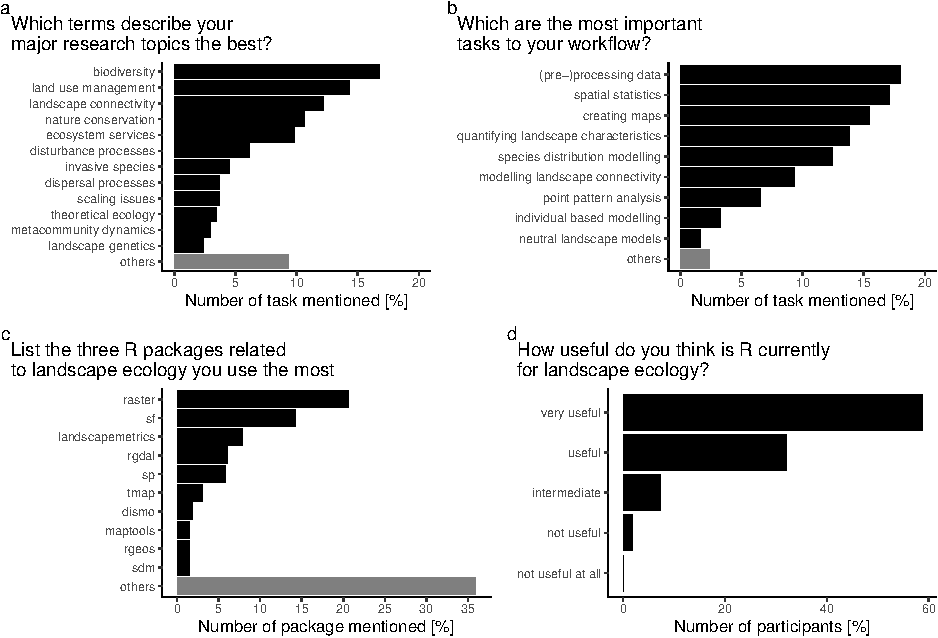
\includegraphics{paper_files/figure-latex/fig-survey-1} 

}

\caption{Results of the online survey about open-source software tools in R for landscape ecology. Results include A) which terms describe major reserach topics the best, B) the most important workflow task, C) the most used R packages and D) the overall usefulnes or R for landscape ecology. 'others' includes all answers with less than five total mentions.}\label{fig:fig-survey}
\end{figure}

\FloatBarrier

\hypertarget{missing-packages}{%
\section{Missing packages}\label{missing-packages}}

The survey also included a section in which participants could list methods and tools that are currently missing in \emph{R} and answers to this question were very diverse.

Overall, 22.3\% of the participants reported that currently no packages and functionality are missing for them or they lack the overview to answer the question.
There were three most common topics across the answers of the participants.
Firstly, many participants (13.6\%) wished for a better computational performance of \emph{R} in terms of speed and required RAM, especially for larger data.
Secondly, participant are missing specific approaches to quantify landscape characteristics (such as surface metrics), or are wishing for an improvement of currently available approaches to quantify landscape characteristics (9.7\%).
Thirdly, many participants (8.7\%) are currently missing advanced and easy-to-apply methods to create high-quality maps or other visualization-related functionality.

\hypertarget{conclusions}{%
\section{Conclusions}\label{conclusions}}

Since its first introduction in 1995, \emph{R} has come a long way from a statistical programming language to a powerful tool for landscape ecology.
Today, many \emph{R} packages, mainly developed by the community itself, provide a vast collection of functions and algorithms aimed for spatial data handling and analysis.
The highly dynamic development of \emph{R} packages for landscape ecology also shows the strength of open-source software with its high innovation, transparency, reliability, and longevity.
However, since the scientific field of landscape ecology constantly changes and improves, also the \emph{R} programming language and its packages need to change and adapt these changes.

\bibliographystyle{spphys}
\bibliography{bibliography.bib}

\end{document}
